\documentclass{article}\usepackage[]{graphicx}\usepackage[]{color}
%% maxwidth is the original width if it is less than linewidth
%% otherwise use linewidth (to make sure the graphics do not exceed the margin)
\makeatletter
\def\maxwidth{ %
  \ifdim\Gin@nat@width>\linewidth
    \linewidth
  \else
    \Gin@nat@width
  \fi
}
\makeatother

\definecolor{fgcolor}{rgb}{0.345, 0.345, 0.345}
\newcommand{\hlnum}[1]{\textcolor[rgb]{0.686,0.059,0.569}{#1}}%
\newcommand{\hlstr}[1]{\textcolor[rgb]{0.192,0.494,0.8}{#1}}%
\newcommand{\hlcom}[1]{\textcolor[rgb]{0.678,0.584,0.686}{\textit{#1}}}%
\newcommand{\hlopt}[1]{\textcolor[rgb]{0,0,0}{#1}}%
\newcommand{\hlstd}[1]{\textcolor[rgb]{0.345,0.345,0.345}{#1}}%
\newcommand{\hlkwa}[1]{\textcolor[rgb]{0.161,0.373,0.58}{\textbf{#1}}}%
\newcommand{\hlkwb}[1]{\textcolor[rgb]{0.69,0.353,0.396}{#1}}%
\newcommand{\hlkwc}[1]{\textcolor[rgb]{0.333,0.667,0.333}{#1}}%
\newcommand{\hlkwd}[1]{\textcolor[rgb]{0.737,0.353,0.396}{\textbf{#1}}}%
\let\hlipl\hlkwb

\usepackage{framed}
\makeatletter
\newenvironment{kframe}{%
 \def\at@end@of@kframe{}%
 \ifinner\ifhmode%
  \def\at@end@of@kframe{\end{minipage}}%
  \begin{minipage}{\columnwidth}%
 \fi\fi%
 \def\FrameCommand##1{\hskip\@totalleftmargin \hskip-\fboxsep
 \colorbox{shadecolor}{##1}\hskip-\fboxsep
     % There is no \\@totalrightmargin, so:
     \hskip-\linewidth \hskip-\@totalleftmargin \hskip\columnwidth}%
 \MakeFramed {\advance\hsize-\width
   \@totalleftmargin\z@ \linewidth\hsize
   \@setminipage}}%
 {\par\unskip\endMakeFramed%
 \at@end@of@kframe}
\makeatother

\definecolor{shadecolor}{rgb}{.97, .97, .97}
\definecolor{messagecolor}{rgb}{0, 0, 0}
\definecolor{warningcolor}{rgb}{1, 0, 1}
\definecolor{errorcolor}{rgb}{1, 0, 0}
\newenvironment{knitrout}{}{} % an empty environment to be redefined in TeX

\usepackage{alltt}

% \usepackage[utf8]{inputenc}
\usepackage{amsmath}
\usepackage{fancyhdr}
\usepackage{array}
\usepackage{longtable}
\usepackage{graphicx}
\usepackage{color}
\usepackage[letterpaper, margin=1in]{geometry}
\usepackage{lscape}
\newcommand{\blandscape}{\begin{landscape}}
\newcommand{\elandscape}{\end{landscape}}
\usepackage{dcolumn}
\usepackage{bbm}
\usepackage{threeparttable}
\usepackage{booktabs}
\usepackage{expex}
\usepackage{pdflscape}
\usepackage{rotating, graphicx}
\usepackage{tabulary}
\usepackage{lscape}
\usepackage{makecell}
\usepackage{algorithm}
\usepackage{multirow}
\usepackage{colortbl}
\usepackage{longtable}
\usepackage{array}
\usepackage{multirow}
\usepackage{wrapfig}
\usepackage{float}
\usepackage{pdflscape}
\usepackage{tabu}
\usepackage{threeparttable}

\title{%
Homework 7\\
\large Applied Mutlivariate Analysis}
\date{October 22, 2018}
\author{Emorie Beck}
\IfFileExists{upquote.sty}{\usepackage{upquote}}{}
\begin{document}
\maketitle
% \SweaveOpts{concordance=TRUE}

\section{Workspace}
\subsection{Packages}



\begin{knitrout}
\definecolor{shadecolor}{rgb}{0.969, 0.969, 0.969}\color{fgcolor}\begin{kframe}
\begin{alltt}
\hlkwd{library}\hlstd{(car)}
\hlkwd{library}\hlstd{(knitr)}
\hlkwd{library}\hlstd{(psych)}
\hlkwd{library}\hlstd{(gridExtra)}
\hlkwd{library}\hlstd{(knitr)}
\hlkwd{library}\hlstd{(kableExtra)}
\hlkwd{library}\hlstd{(MASS)}
\hlkwd{library}\hlstd{(vegan)}
\hlkwd{library}\hlstd{(smacof)}
\hlkwd{library}\hlstd{(scatterplot3d)}
\hlkwd{library}\hlstd{(ape)}
\hlkwd{library}\hlstd{(ade4)}
\hlkwd{library}\hlstd{(ecodist)}
\hlkwd{library}\hlstd{(cluster)}
\hlkwd{library}\hlstd{(factoextra)}
\hlkwd{library}\hlstd{(ggdendro)}
\hlkwd{library}\hlstd{(lme4)}
\hlkwd{library}\hlstd{(plyr)}
\hlkwd{library}\hlstd{(tidyverse)}
\end{alltt}
\end{kframe}
\end{knitrout}



\subsection{data}
I’ve just obtained a zoo! Well, at least all of the animals from a zoo; the land was lost because of failure to pay property taxes and the owner decided to get out of the zoo business. I’ve always wanted to own a zoo, but I don’t know beans about it. My first job is to organize the creatures in some sensible way so that the staff can care for them easily and visitors can find what they want to see without too much random walking around.

The file, Set\_6.csv, contains one animal per row. The columns are 20 different features that define the animals. All are self-explanatory except the last one (catsize). This is an indicator of whether the animal is smaller than a typical housecat or larger than a typical housecat. All variables are binary with 0 indicating the absence of the feature (e.g., does not produce milk) and 1 indicating the presence of the feature (e.g., has fins).

\begin{knitrout}
\definecolor{shadecolor}{rgb}{0.969, 0.969, 0.969}\color{fgcolor}\begin{kframe}
\begin{alltt}
\hlstd{wd} \hlkwb{<-} \hlstr{"https://github.com/emoriebeck/homeworks/raw/master/multivariate/homeworks/homework8"}

\hlstd{dat} \hlkwb{<-} \hlkwd{sprintf}\hlstd{(}\hlstr{"%s/Set_6(1).csv"}\hlstd{, wd)} \hlopt
  \hlkwd{read.csv}\hlstd{(.,} \hlkwc{stringsAsFactors} \hlstd{= F)}

\hlkwd{head}\hlstd{(dat)}
\end{alltt}
\begin{verbatim}
##   hair feathers eggs milk airborne aquatic predator toothed backbone
## 1    1        0    0    1        0       0        1       1        1
## 2    1        0    0    1        0       0        0       1        1
## 3    0        0    1    1        0       1        1       1        1
## 4    1        0    0    1        0       0        1       1        1
## 5    1        0    0    1        0       0        1       1        1
## 6    1        0    0    1        0       0        0       1        1
##   breathes venomous fins two_legs four_legs five_legs six_legs eight_legs
## 1        1        0    0        0         1         0        0          0
## 2        1        0    0        0         1         0        0          0
## 3        0        0    1        0         0         0        0          0
## 4        1        0    0        0         1         0        0          0
## 5        1        0    0        0         1         0        0          0
## 6        1        0    0        0         1         0        0          0
##   tail domestic catsize
## 1    0        0       1
## 2    1        0       1
## 3    1        0       0
## 4    0        0       1
## 5    1        0       1
## 6    1        0       1
\end{verbatim}
\end{kframe}
\end{knitrout}

\section{Question 1}
Analyze these data using each of the following hierarchical clustering procedures: single linkage, complete linkage, average linkage, centroid method, Ward’s method.

\begin{knitrout}
\definecolor{shadecolor}{rgb}{0.969, 0.969, 0.969}\color{fgcolor}\begin{kframe}
\begin{alltt}
\hlcom{# create a fucntion for creating the dendrograms}
\hlstd{plot_fun} \hlkwb{<-} \hlkwa{function}\hlstd{(}\hlkwc{cl}\hlstd{,} \hlkwc{m}\hlstd{)\{}
  \hlkwd{ggdendrogram}\hlstd{(cl,}\hlkwc{theme_dendro}\hlstd{=}\hlnum{FALSE}\hlstd{,}\hlkwc{size}\hlstd{=}\hlnum{4}\hlstd{)} \hlopt{+}
    \hlkwd{labs}\hlstd{(}\hlkwc{x} \hlstd{=} \hlstr{"Objects"}\hlstd{,} \hlkwc{y} \hlstd{=} \hlstr{"Heights"}\hlstd{,} \hlkwc{title} \hlstd{= m)} \hlopt{+}
    \hlkwd{theme_classic}\hlstd{()} \hlopt{+}
    \hlkwd{theme}\hlstd{(}\hlkwc{plot.title} \hlstd{=} \hlkwd{element_text}\hlstd{(}\hlkwc{face} \hlstd{=} \hlstr{"bold"}\hlstd{,} \hlkwc{hjust} \hlstd{=} \hlnum{.5}\hlstd{))}
\hlstd{\}}

\hlstd{nested.mods} \hlkwb{<-} \hlkwd{tribble}\hlstd{(}
  \hlopt{~}\hlstd{method_arg,} \hlopt{~}\hlstd{Method,} \hlopt{~}\hlstd{data,}
  \hlstr{"single"}\hlstd{,} \hlstr{"Single Linkage"}\hlstd{, dat,}
  \hlstr{"complete"}\hlstd{,}  \hlstr{"Complete Linkage"}\hlstd{, dat,}
  \hlstr{"average"}\hlstd{,} \hlstr{"Average Linkage"}\hlstd{, dat,}
  \hlstr{"centroid"}\hlstd{,} \hlstr{"Centroid Method"}\hlstd{, dat,}
  \hlstr{"ward.D2"}\hlstd{,} \hlstr{"Ward's Method"}\hlstd{, dat}
\hlstd{)} \hlopt
  \hlkwd{mutate}\hlstd{(}\hlkwc{dist} \hlstd{=} \hlkwd{map}\hlstd{(data,} \hlopt{~}\hlstd{(}\hlkwd{dist}\hlstd{(.,}\hlkwc{method}\hlstd{=}\hlstr{"euclidean"}\hlstd{))}\hlopt{^}\hlnum{2}\hlstd{),}
         \hlkwc{cl} \hlstd{=} \hlkwd{map2}\hlstd{(dist, method_arg,} \hlopt{~}\hlkwd{hclust}\hlstd{(.x,} \hlkwc{method}\hlstd{=.y)),}
         \hlkwc{merge} \hlstd{=} \hlkwd{map}\hlstd{(cl,} \hlopt{~}\hlkwd{data.frame}\hlstd{(.}\hlopt{$}\hlstd{merge)),}
         \hlkwc{pl} \hlstd{=} \hlkwd{map2}\hlstd{(cl, Method, plot_fun))}

\hlcom{# merges}
\hlstd{nested.mods} \hlopt \hlkwd{unnest}\hlstd{(merge)} \hlopt
  \hlkwd{group_by}\hlstd{(Method)} \hlopt
  \hlkwd{mutate}\hlstd{(}\hlkwc{m_num} \hlstd{=} \hlnum{1}\hlopt{:}\hlkwd{n}\hlstd{())} \hlopt
  \hlkwd{gather}\hlstd{(}\hlkwc{key} \hlstd{= x,} \hlkwc{value} \hlstd{= value, X1, X2)} \hlopt
  \hlkwd{select}\hlstd{(}\hlopt{-}\hlstd{method_arg)} \hlopt
  \hlkwd{unite}\hlstd{(tmp, Method, x,} \hlkwc{sep} \hlstd{=} \hlstr{"."}\hlstd{)} \hlopt
  \hlkwd{spread}\hlstd{(tmp, value)}
\end{alltt}
\begin{verbatim}
## # A tibble: 100 x 11
##    m_num `Average Linkag~ `Average Linkag~ `Centroid Metho~
##    <int>            <int>            <int>            <int>
##  1     1               -1               -4               -1
##  2     2               -2               -6               -2
##  3     3              -18                2              -18
##  4     4              -23                3              -23
##  5     5              -29                4              -29
##  6     6              -56                5              -56
##  7     7               -5              -11               -5
##  8     8              -45                7              -45
##  9     9              -46                8              -46
## 10    10              -48                9              -48
## # ... with 90 more rows, and 7 more variables: `Centroid Method.X2` <int>,
## #   `Complete Linkage.X1` <int>, `Complete Linkage.X2` <int>, `Single
## #   Linkage.X1` <int>, `Single Linkage.X2` <int>, `Ward's
## #   Method.X1` <int>, `Ward's Method.X2` <int>
\end{verbatim}
\begin{alltt}
\hlkwd{do.call}\hlstd{(}\hlstr{"grid.arrange"}\hlstd{, nested.mods}\hlopt{$}\hlstd{pl)}
\end{alltt}
\end{kframe}
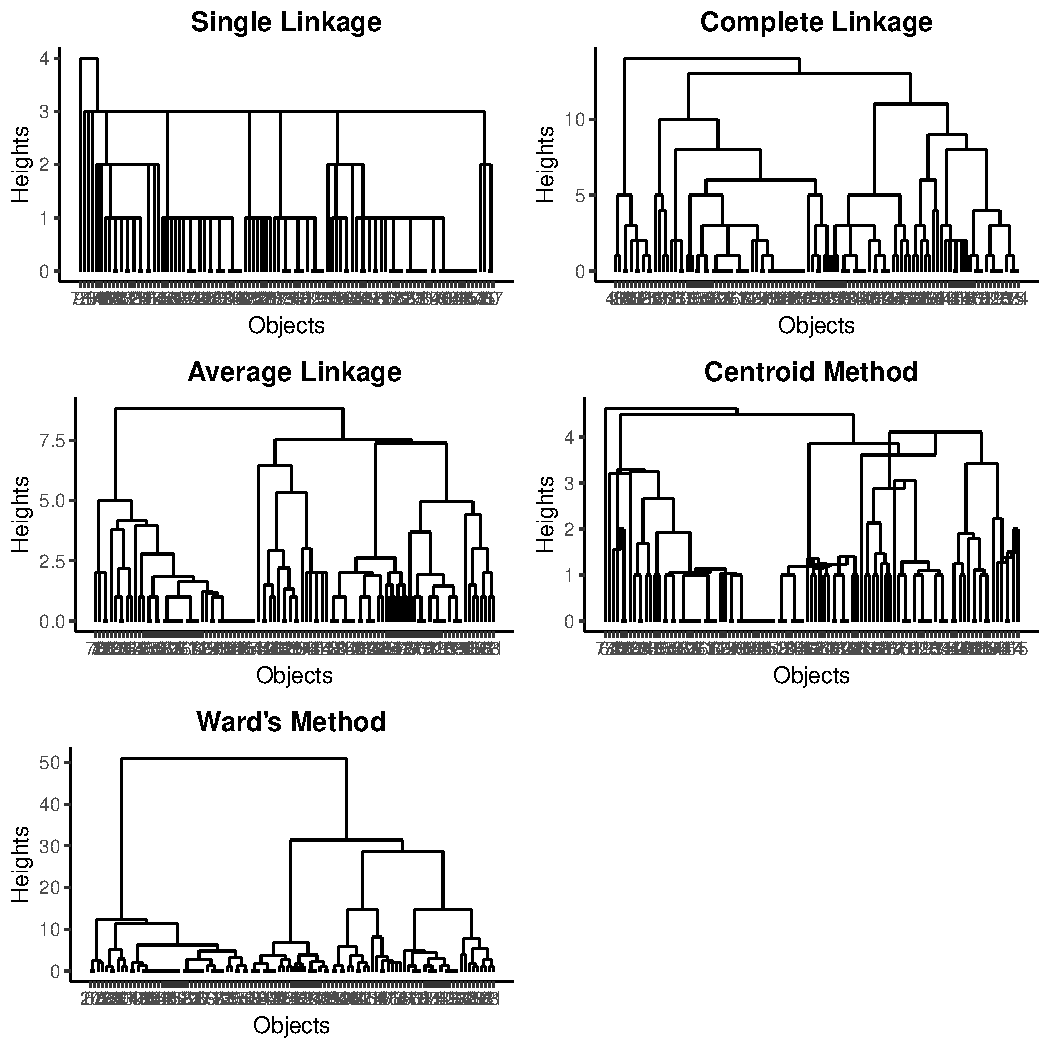
\includegraphics[width=\maxwidth]{figure/unnamed-chunk-4-1} 

\end{knitrout}

\section{Question 2}
Choose the method that you believe provides the easiest interpretation of the data. Based on that method, how many sections or major areas do I need to build in my zoo so that I can house similar animals together? Provide a justification for this conclusion.

In this case, Ward's Method appears to provide the most interpretable clusters, suggesting 3 clusters before you start seeing greater losses in accuracy.

\begin{knitrout}
\definecolor{shadecolor}{rgb}{0.969, 0.969, 0.969}\color{fgcolor}\begin{kframe}
\begin{alltt}
\hlstd{new.dat} \hlkwb{<-} \hlstd{dat}
\hlstd{new.dat}\hlopt{$}\hlstd{clustnumber} \hlkwb{<-} \hlkwd{cutree}\hlstd{((nested.mods} \hlopt \hlkwd{filter}\hlstd{(method_arg} \hlopt{==} \hlstr{"ward.D2"}\hlstd{))}\hlopt{$}\hlstd{cl[[}\hlnum{1}\hlstd{]],} \hlkwc{k}\hlstd{=}\hlnum{3}\hlstd{)}
\end{alltt}
\end{kframe}
\end{knitrout}


\section{Question 3}
Based on the dominant features of the clusters you have identified, try to name the major clusters.

\begin{knitrout}
\definecolor{shadecolor}{rgb}{0.969, 0.969, 0.969}\color{fgcolor}\begin{kframe}
\begin{alltt}
\hlstd{new.dat} \hlopt \hlkwd{gather}\hlstd{(feature, value,} \hlopt{-}\hlstd{clustnumber)} \hlopt
  \hlkwd{filter}\hlstd{(value} \hlopt{==} \hlnum{1}\hlstd{)} \hlopt
  \hlkwd{group_by}\hlstd{(clustnumber, feature)} \hlopt
  \hlkwd{summarize}\hlstd{(}\hlkwc{prop} \hlstd{=} \hlkwd{n}\hlstd{()}\hlopt{/}\hlnum{40}\hlstd{)} \hlopt
  \hlkwd{spread}\hlstd{(clustnumber, prop)} \hlopt
  \hlkwd{arrange}\hlstd{(}\hlkwd{desc}\hlstd{(`1`),} \hlkwd{desc}\hlstd{(`2`),} \hlkwd{desc}\hlstd{(`3`))} \hlopt
  \hlkwd{kable}\hlstd{(.,} \hlstr{"latex"}\hlstd{,} \hlkwc{booktab} \hlstd{= T,} \hlkwc{digits} \hlstd{=} \hlnum{2}\hlstd{)} \hlopt
  \hlkwd{kable_styling}\hlstd{(}\hlkwc{full_width} \hlstd{= F)} \hlopt
  \hlkwd{add_footnote}\hlstd{(}\hlstr{"Note: values represent propotions of across each of the features within a cluster"}\hlstd{)}
\end{alltt}
\end{kframe}\begin{table}[H]
\centering
\begin{tabular}{lrrr}
\toprule
feature & 1 & 2 & 3\\
\midrule
backbone & 1.00 & 0.57 & 0.50\\
toothed & 1.00 & 0.52 & NA\\
breathes & 1.00 & 0.50 & 0.50\\
milk & 1.00 & 0.05 & NA\\
hair & 0.95 & 0.12 & NA\\
\addlinespace
tail & 0.85 & 0.52 & 0.50\\
catsize & 0.78 & 0.18 & 0.15\\
four\_legs & 0.75 & 0.20 & NA\\
predator & 0.52 & 0.65 & 0.22\\
domestic & 0.20 & 0.05 & 0.08\\
\addlinespace
two\_legs & 0.18 & NA & 0.50\\
aquatic & 0.12 & 0.62 & 0.15\\
fins & 0.10 & 0.32 & NA\\
airborne & 0.05 & 0.15 & 0.40\\
eggs & NA & 0.98 & 0.50\\
\addlinespace
six\_legs & NA & 0.25 & NA\\
venomous & NA & 0.20 & NA\\
eight\_legs & NA & 0.05 & NA\\
five\_legs & NA & 0.02 & NA\\
feathers & NA & NA & 0.50\\
\bottomrule
\multicolumn{4}{l}{\textsuperscript{a} Note: values represent propotions}\\
\multicolumn{4}{l}{of across each of the features}\\
\multicolumn{4}{l}{within a cluster}\\
\end{tabular}
\end{table}


\end{knitrout}

Based on this, it appears the first cluster is mammals, the second is amphibians and water animals, and the third are birds.

\section{Question 4}
Just for fun. I am really going to get in trouble for one of the animals I will have in my zoo. The previous owner gave me a big discount on the animal collection provided I take this one, which was causing him all kinds of grief. Can you identify it?

\begin{knitrout}
\definecolor{shadecolor}{rgb}{0.969, 0.969, 0.969}\color{fgcolor}\begin{kframe}
\begin{alltt}
\hlstd{case} \hlkwb{<-} \hlstd{(dat} \hlopt
  \hlkwd{mutate}\hlstd{(}\hlkwc{casenum} \hlstd{=} \hlnum{1}\hlopt{:}\hlkwd{n}\hlstd{())} \hlopt
  \hlkwd{filter}\hlstd{(predator} \hlopt{==} \hlnum{1} \hlopt{&} \hlstd{toothed} \hlopt{==} \hlnum{1} \hlopt{&} \hlstd{domestic} \hlopt{==} \hlnum{0} \hlopt{&} \hlstd{catsize} \hlopt{==} \hlnum{1} \hlopt{&} \hlstd{venomous} \hlopt{==} \hlnum{1}\hlstd{))}\hlopt{$}\hlstd{casenum}
\end{alltt}
\end{kframe}
\end{knitrout}

Based on this, case \# 87 is likely to cause all kinds of grief. 


\end{document}
